\subsubsection{Árboles de decisión}

	Un árbol de decisión es un modelo predictivo que sirve para representar y categorizar una serie de condiciones que ocurren de manera sucesiva, para la resolución de un problema. Pueden ser usados para la clasificación(variables discretas) o regresión(variables continuas). Es una estructura simple donde los nodos no terminales representan pruebas en uno o más atributos o características y los nodos terminales reflejan las decisiones. El árbol común consiste de una raiz, ramas, nodos(lugares donde las ramas se dividen) y hojas. En los árboles de decisión para clasificación, cada nodo del árbol representa una característica, cada rama que sale de un nodo representa un valor posible para la característica que representa al nodo y por último las hojas representan la etiqueta de clase(decisión tomada luego de computar todas las características). La clasificación comienza en el nodo raiz, donde se pregunta sobre algun valor de una característica en particular del objeto a analizar. Las diferentes ramas que salen del nodo raiz corresponden a las diferentes valores posibles. Basado en la respuesta se continua por la rama hasta el nodo siguiente. La siguiente etapa es realizar una decisión en el nodo en cuestión que puede ser considerado como la raiz del sub-árbol. Se continua de esta manera hasta que se alcanza un nodo hoja, el cual no contiene mas preguntas. Cada nodo hoja contiene una etiqueta categórica y al objeto se le asigna la etiqueta del nodo hoja que ha alcanzado. Un ejemplo simple se puede observar en la figura \ref{fig: Arbol de decision} donde se representa el problema de si es conveniente ir a jugar al tenis basándose en las características del clima.
		\begin{figure}[htbp]
			\centering
			\fbox{ 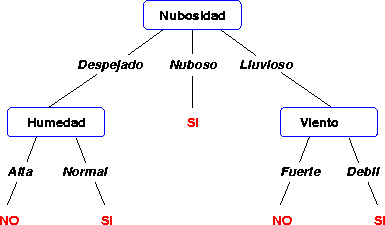
\includegraphics[scale=0.5]{img/tenis_decision_tree.png} }
			\caption{Árbol de decisión.}
			\label{fig: Arbol de decision}
		\end{figure} 
	